\chapter{Strukturaufklärung der Chl-Kataboliten mit ESI-MS}

\section{Identifizierte Chl-Kataboliten}

\subsection{Bo-DYCC}

\begin{figure}[!htbp]
  \centering
  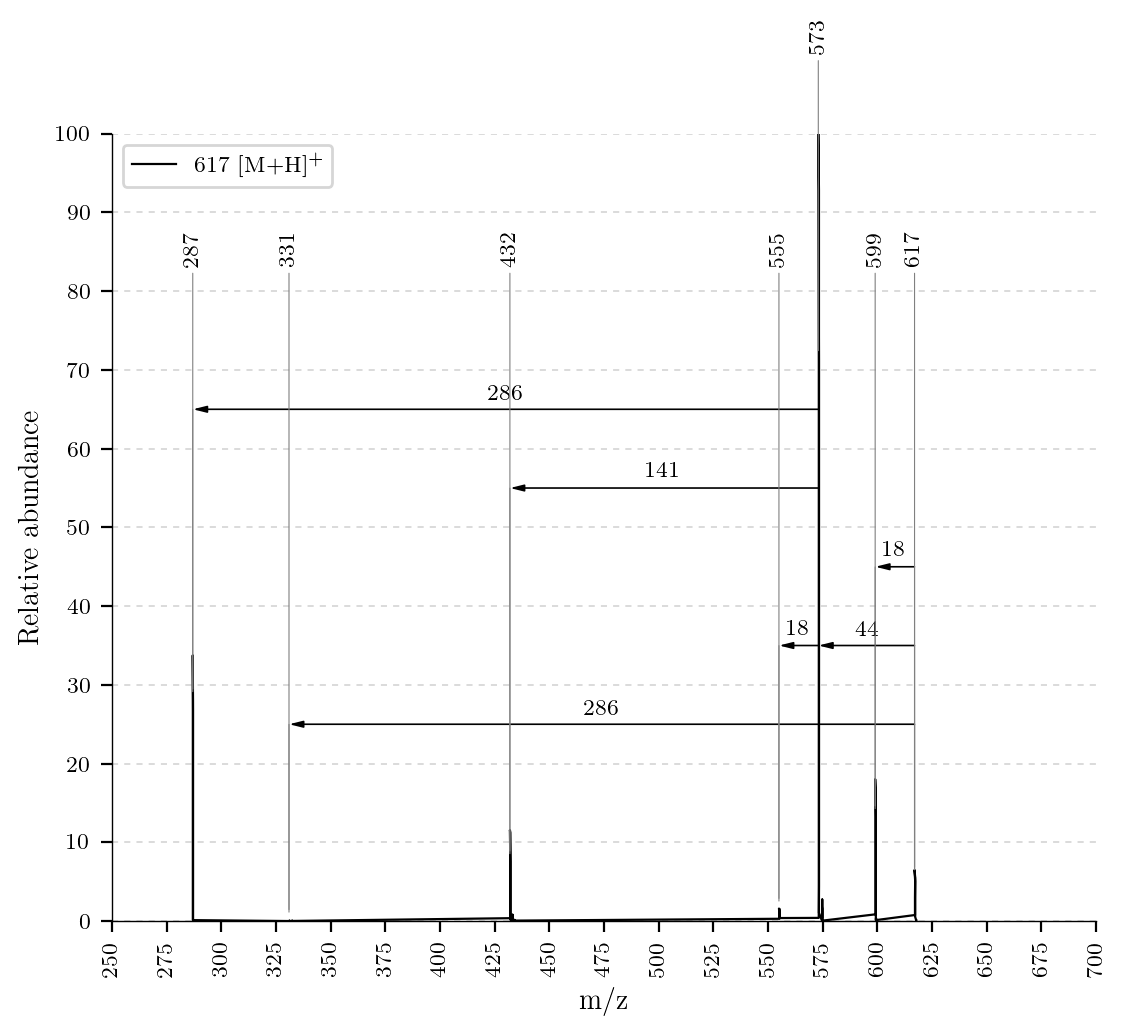
\includegraphics[width=\textwidth, height=0.7\textwidth]{figures/Kapitel7/Kataboliten/VWA_MS_617.png}
  \caption[ESI-MS Spektrum von Bo-DYCC, Quelle: Autor]{ESI-MS Spektrum von Bo-DYCC mit m/z = 617 [M+H]\textsuperscript{+} und den Abspaltungen}
  \label{fig:617MH}
\end{figure}

Dieser \gls{Chl-K} konnte mit der Methode von MS Leafspray nicht gefunden werden. Mit einem hochauflösenden Massenspektrometer konnte er mit m/z = 617 [M+H]\textsuperscript{+} identifiziert werden. Er zeigt Abspaltungen von \ch{H2O} bei m/z = 599 [M - (\ch{H2O}) + H]\textsuperscript{+} , von \ch{CO2} bei m/z = 573 [M - (\ch{CO2}) + H]\textsuperscript{+}, von Ring A bei m/z = 432 [M - (Ring A) + H]\textsuperscript{+} und von Ring C und D bei m/z = 331 [M - (Ring C, Ring D) + H]\textsuperscript{+} (Abbildung \ref{fig:617MH}).

Die Struktur des Bo-DYCC  wird wie in Abbildung \ref{fig:617MHStruktur} vorgeschlagen. Aufgrund der \ch{CO2} Abspaltung wird eine freie Carbonsäure an Position .. angenommen. Die zwei fehlenden H-Atomen im Vergleich zum Bo-DNCC und die sinnvollen Zuordnungen der anderen Fragmentierungen weisen auf eine Doppelbindung an Position .. hin. Es wird vermutet, dass er eine Vorstufe zum Bo-DNCC darstellt. 

Der Mechanismus der Abspaltung von Ring C zusammen mit Ring D wird wie in den Abbildungen \ref{fig:617MHElectronMovement} und \ref{fig:331MH} dargestellt angenommen. 

\begin{figure}[!htbp]
  \centering
  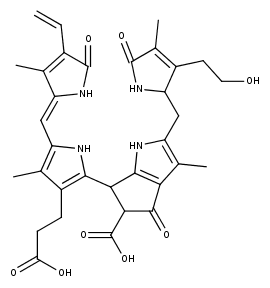
\includegraphics[scale=0.6]{figures/Kapitel7/Kataboliten/fragmentation_structures/VWA_Katabolit_617.png}
  \caption[Strukturvorschlag von Bo-DYCC, Quelle: Autor]{Strukturvorschlag von Bo-DYCC mit Summenformel \ch{C33H36N4O8}}
  \label{fig:617MHStruktur}
\end{figure}

\begin{figure}[!htbp]
  \begin{subfigure}[b]{0.5\textwidth}
    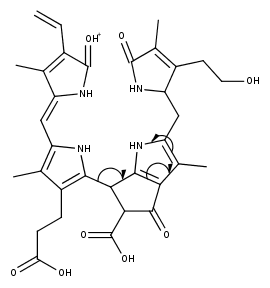
\includegraphics[width=\textwidth]{figures/Kapitel7/Kataboliten/fragmentation_structures/VWA_Katabolit_617_MH_RingD-RingC_331_electronMovement.png}
    \caption{}
    \label{fig:617MHElectronMovement}
  \end{subfigure}
  \hfill
  \begin{subfigure}[b]{0.5\textwidth}
    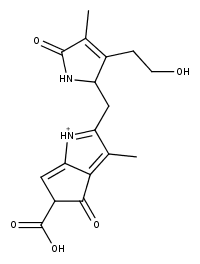
\includegraphics[width=\textwidth]{figures/Kapitel7/Kataboliten/fragmentation_structures/VWA_Katabolit_617-RingD-RingC_331.png}
    \caption{}
    \label{fig:331MH}
  \end{subfigure}
  \caption[Abspaltungsmechanismus von Ring C und Ring D bei Bo-DYCC, Quelle: Autor]{mechanistischer Vorschlag für die Abspaltung von Ring C und Ring D: (a) vorgeschlagene Bewegung der Elektronen, (b) Resultat der Abspaltung bei m/z = 331 [M - (Ring C, Ring D) + H]\textsuperscript{+} und Summenformel \ch{}}
\end{figure}

\subsection{Bo-DNCC}

Vom Bo-DNCC wurde mit dieser Methode nur die protonierte Verbindung bei m/z = 619 [M+H]\textsuperscript{+} aufgenommen. Sie zeigt Abspaltungen von \ch{H2O} bei m/z = 601, von \ch{CO2} bei m/z = 575, von Ring D bei m/z = 452 und eine gemeinsame Abspaltung von Ring D und Ring A bei m/z = 311 (Abbildung \ref{fig:619MH}. 

\begin{figure}[!htbp]
  \centering
  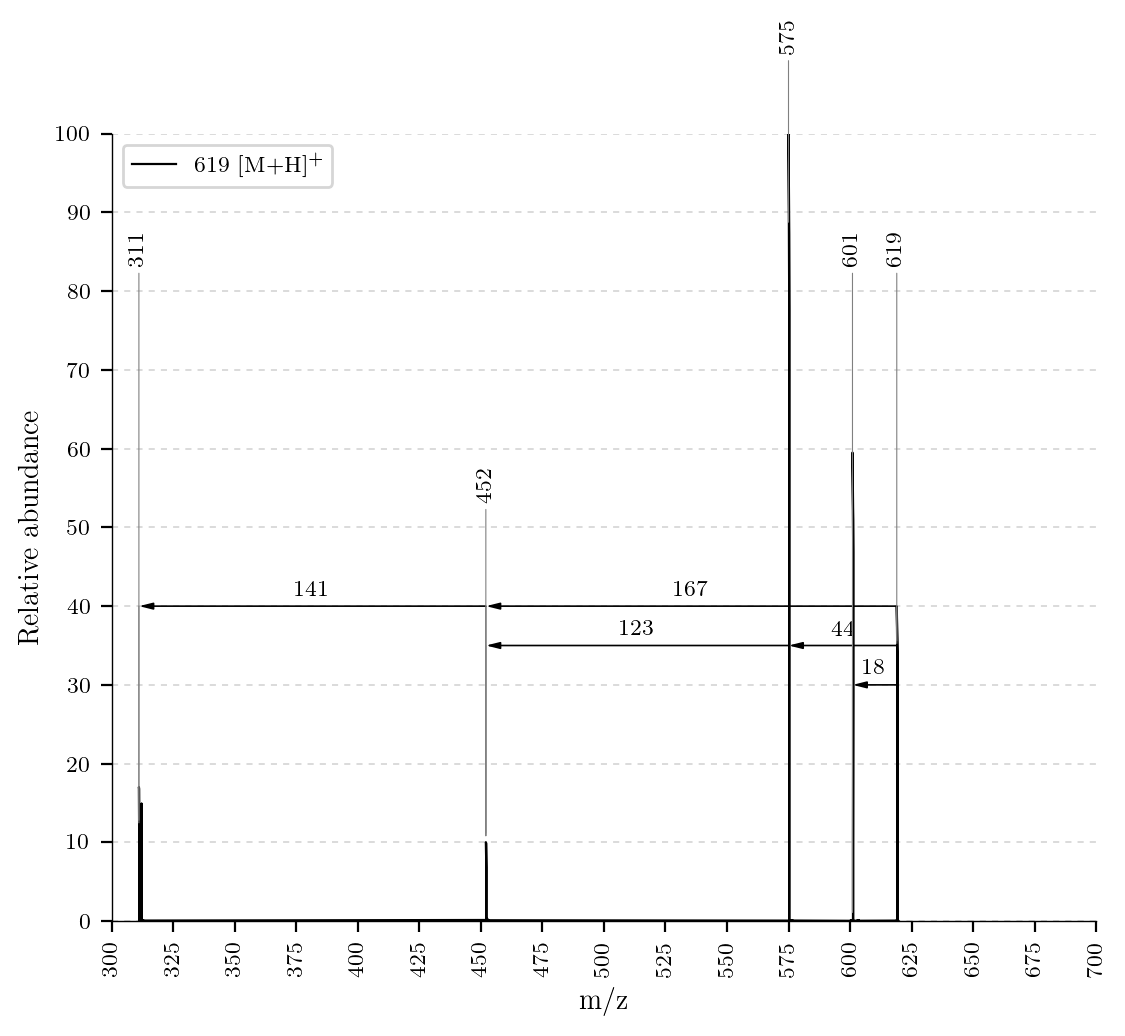
\includegraphics[width=\textwidth, height=0.7\textwidth]{figures/Kapitel7/Kataboliten/VWA_MS_619.png}
  \caption[ESI-MS Spektrum von Bo-DNCC, Quelle: Autor]{ESI-MS Spektrum von Bo-DNCC bei m/z = 619 }
  \label{fig:619MH}
\end{figure}

Da für die Abspaltung von Ring A und Ring D jeweils ein Mechanismus in \cite{StructureElucidation} vorgeschlagen wird, gibt es unterschiedliche Möglichkeiten für das Abspaltungsprodukt, wenn wie hier beobachtet beide gleichzeitig abgespalten werden (Mechanismus Abbildung \ref{fig:619MHElectronMovement}). In den Abbildungen \ref{fig:311MHMesomer1}, \ref{fig:311MHMesomer2}-b werden die einzelnen Mesomere vorgeschlagen. Als stabiler werden die Mesomere bei \ref{fig:311MHMesomer2}-b aufgrund des stabilen konjugierten Systems erachtet.

\begin{figure}[!htbp]
  \begin{subfigure}[b]{0.5\textwidth}
    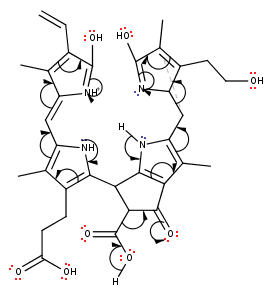
\includegraphics[width=\textwidth]{figures/Kapitel7/Kataboliten/fragmentation_structures/VWA_Katabolit_619_MH-CO2-RingA-RIngD_311_electronMovement.png}
    \caption{}
    \label{fig:619MHElectronMovement}
  \end{subfigure}
  \hfill
  \begin{subfigure}[b]{0.5\textwidth}
    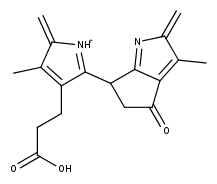
\includegraphics[width=\textwidth]{figures/Kapitel7/Kataboliten/fragmentation_structures/VWA_Katabolit_619-CO2-RingA-RingD_311.png}
    \caption{}
    \label{fig:311MHMesomer1}
  \end{subfigure}
  \caption[Abspaltungsmechanismus von Ring D und Ring A, Quelle: Autor]{vorgeschlagener Abspaltungsmechanismus von Ring D und Ring A: (a) Elektronenbewegung, (b) 1 Mesomer der Abspaltung mit m/z = 311 und Summenformel \ch{}}
\end{figure}

\begin{figure}[!htbp]
  \begin{subfigure}[b]{0.5\textwidth}
    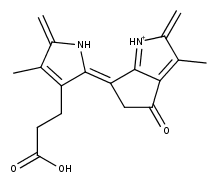
\includegraphics[width=\textwidth]{figures/Kapitel7/Kataboliten/fragmentation_structures/VWA_Katabolit_619-CO2-RingD-RingA_311_Mesomer1.png}
    \caption{}
    \label{fig:311MHMesomer2}
  \end{subfigure}
  \hfill
  \begin{subfigure}[b]{0.5\textwidth}
    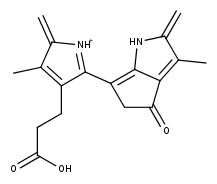
\includegraphics[width=\textwidth]{figures/Kapitel7/Kataboliten/fragmentation_structures/VWA_Katabolit_619-CO2-RingD-RingA_311_Mesomer2.png}
    \caption{}
    \label{fig:311MHMesomer3}
  \end{subfigure}
  \caption[2 Mesomere für potentielle Abspaltungsprodukte von Bo-DNCC, Quelle: Autor]{Mesomere des Abspaltungsproduktes: (a) Mesomer 1, (b) Mesomer 2}
\end{figure}

\subsection{Bo-YCC}

Der Bo-YCC konnte, so wie der Bo-DYCC nicht mit MS Leafspray gefunden werden, dafür jedoch mit der hier verwendeten Methode. Er konnte mit m/z = 645 identifiziert werden und zeigt Abspaltungen von \ch{H2O} bei m/z = 627 und von \ch{CO2} bei m/z = 601 (Abbildung \ref{fig:645MH}). 

\begin{figure}[!htbp]
  \centering
  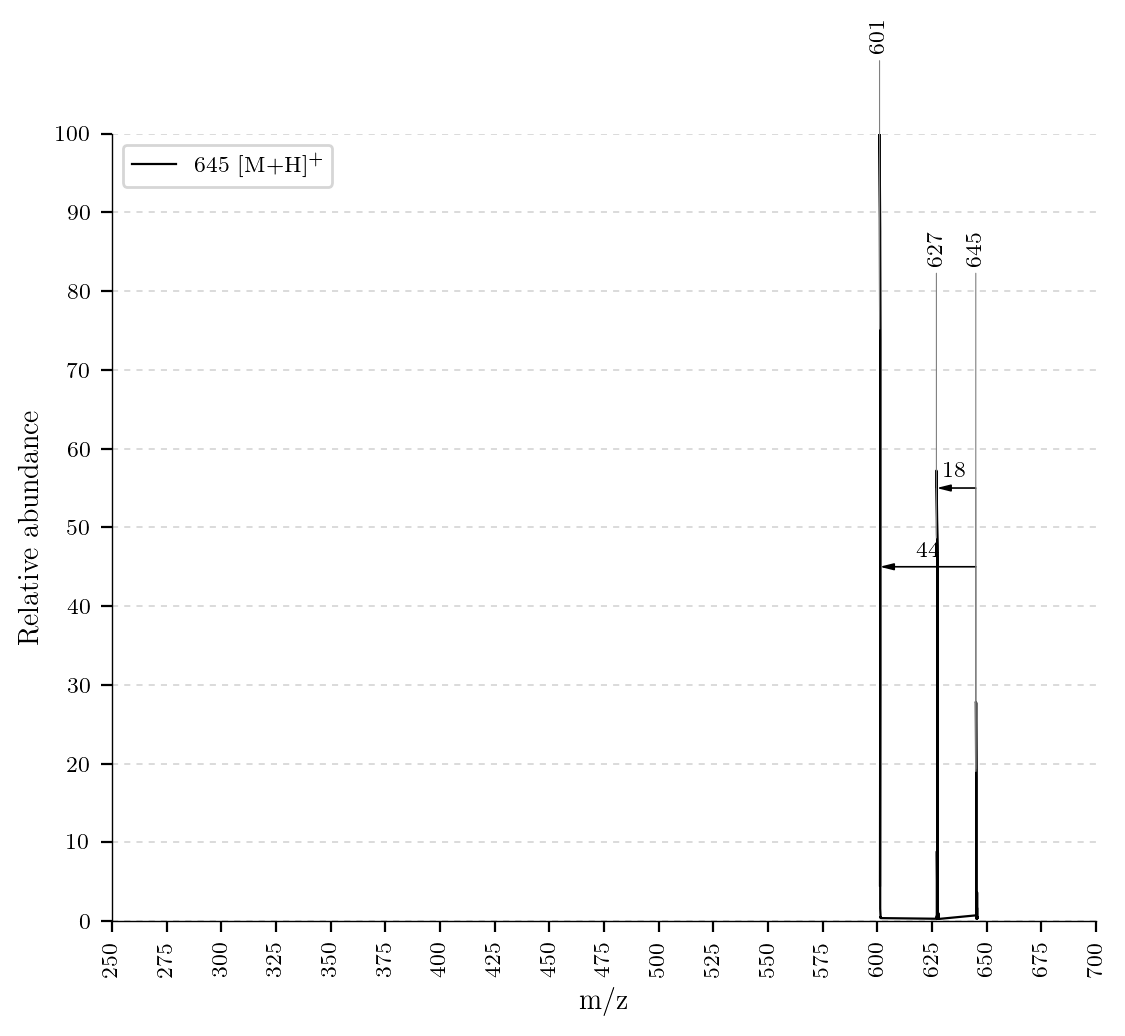
\includegraphics[width=\textwidth, height=0.7\textwidth]{figures/Kapitel7/Kataboliten/VWA_MS_645-1.png}
  \caption[ESI-MS Spektrum von Bo-YCC, Quelle: Autor]{ESI-MS Spektrum von Bo-YCC mit m/z = 645}
  \label{fig:645MH}
\end{figure}

Die Abspaltung von \ch{CO2} hilft, ihn vom Reaktionsprodukt des Bo-DYCC zu unterscheiden. Es wird deswegen an Position .. eine freie Carbonsäure und an Position .. eine Doppelbindung mit einer Hydroxygruppe angenommen (Abbildung \ref{fig:645MStruktur}).

\begin{figure}[!htbp]
  \centering
  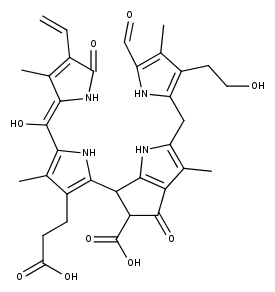
\includegraphics[scale=0.6]{figures/Kapitel7/Kataboliten/fragmentation_structures/VWA_Katabolit_645_vorReaktion.png}
  \caption[Strukturvorschlag von Bo-YCC, Quelle: Autor]{Strukturvorschlag von Bo-YCC mit Summenformel \ch{}}
  \label{fig:645MStruktur}
\end{figure}

\subsection{Bo-NCC-3}

Der Bo-NCC-3 wurde ebenfalls mit MS Leafspray gefunden. Die Masse des \gls{Chl-K} konnte bei m/z = 647 bestimmt werden. Abspaltungen von \ch{H2O} bei m/z = 629, von \ch{CO2} bei m/z = 603 und von Ring D bei m/z = 480 wurden beobachtet. 

Aufgrund der vorgeschlagenen Hydroxygruppe an Position .. wird angenommen, dass das Abspaltungsprodukt in einem Keto-/Enolgleichgewicht steht, wie in Abbildung \ref{fig:480Mechanismus} vorgeschlagen. Mithilfe von Fragmentierungsdiagrammen könnte man argumentieren, dass diese mögliche Tautomerie aufgrund ihrer Stabilität als Triebkraft für die Abspaltung gesehen werden kann.

\begin{figure}[!htbp]
  \centering
  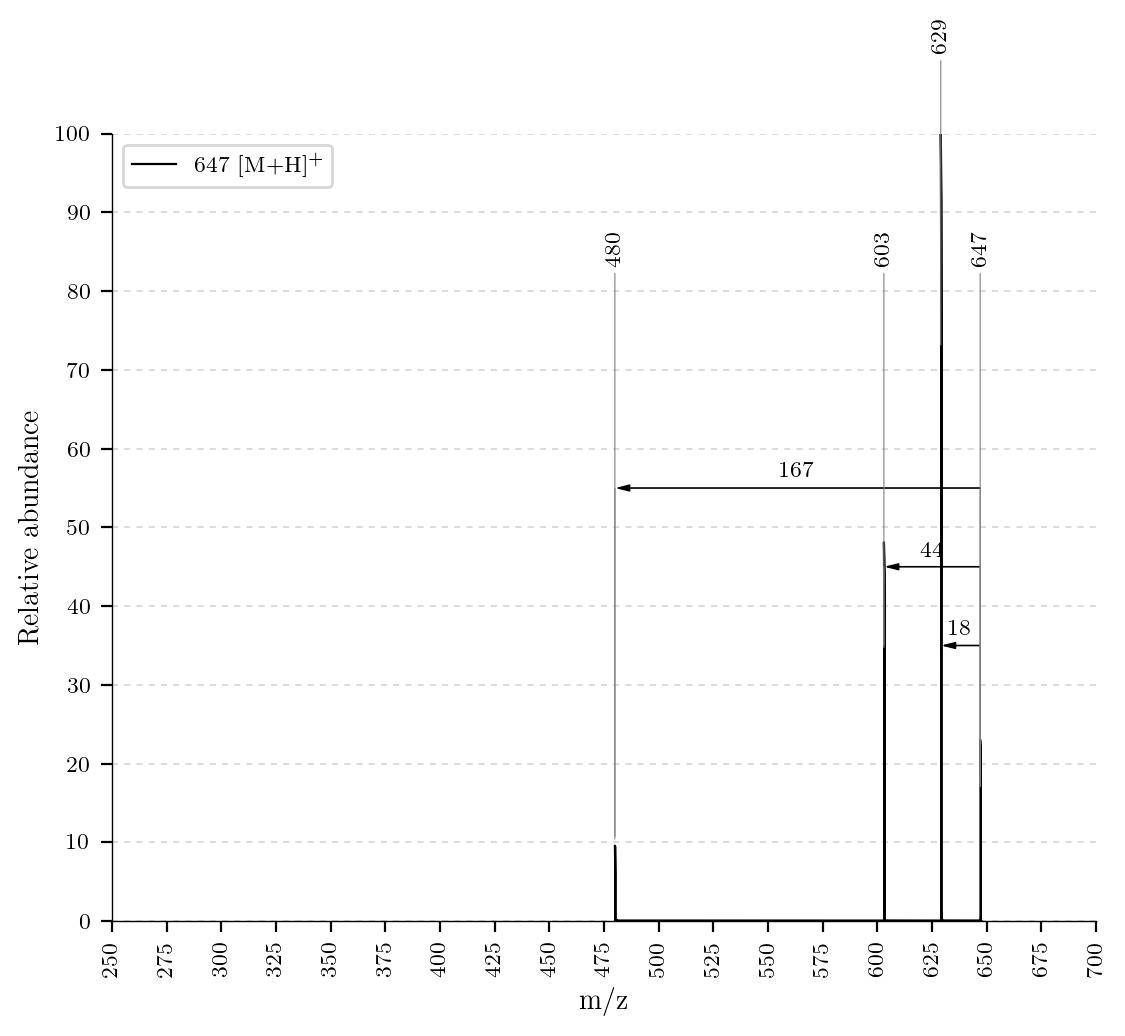
\includegraphics[width=\textwidth, height=0.7\textwidth]{figures/Kapitel7/Kataboliten/VWA_MS_647.png}
  \caption[ESI-MS Spektrum von Bo-NCC-3, Quelle: Autor]{ESI-MS Spektrum von Bo-NCC-3 mit den Abspaltungen}
  \label{fig:647MH}
\end{figure}

\begin{figure}[!htbp]
  \begin{subfigure}[b]{0.5\textwidth}
    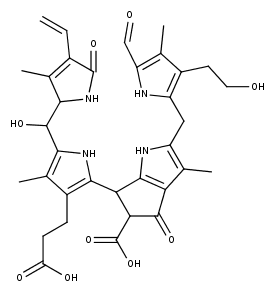
\includegraphics[width=\textwidth]{figures/Kapitel7/Kataboliten/fragmentation_structures/VWA_Katabolit_647.png}
    \caption{}
    \label{fig:647MStruktur}
  \end{subfigure}
  \hfill
  \begin{subfigure}[b]{0.5\textwidth}
    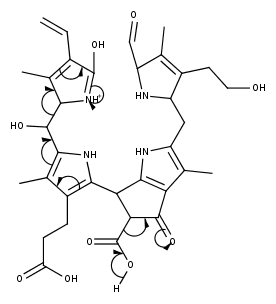
\includegraphics[width=\textwidth]{figures/Kapitel7/Kataboliten/fragmentation_structures/VWA_Katabolit_647-CO2-RingD_480_MH_electronMovement.png}
    \caption{}
    \label{fig:480Mechanismus}
  \end{subfigure}
  \caption[Strukturvorschlag von Bo-NCC-3 und Vorschlag für Mechanismus der Abspaltung von Ring D, Quelle: Autor]{(a) Strukturvorschlag von Bo-NCC-3 mit Summenformel \ch{}, (b) vorgeschlagener Mechanismus für die Abspaltung von Ring D und von \ch{CO2}}
\end{figure}

\begin{figure}[!htbp]
  \begin{subfigure}[b]{0.5\textwidth}
    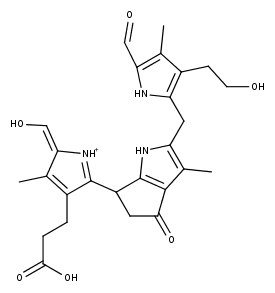
\includegraphics[width=\textwidth]{figures/Kapitel7/Kataboliten/fragmentation_structures/VWA_Katabolit_647-CO2-RingD_480_MH_Enolform.png}
    \caption{}
    \label{fig:NCC2725}
  \end{subfigure}
  \hfill
  \begin{subfigure}[b]{0.5\textwidth}
    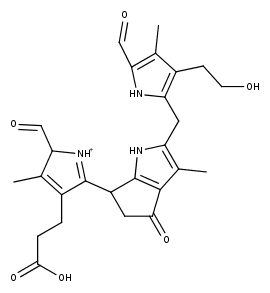
\includegraphics[width=\textwidth]{figures/Kapitel7/Kataboliten/fragmentation_structures/VWA_Katabolit_647-CO2-RingD_480_MH_Ketoform.png}
    \caption{}
    \label{fig:DNCC2991}
  \end{subfigure}
  \caption[vorgeschlagene Keto-/Enoltautomerie der Ring D Abspaltung von Bo-NCC-3, Quelle: Autor]{vorgeschlagene Keto-/Enoltautomerie beim Abspaltungsprodukt von Ring D: (a) Enolform, (b) Aldehyd (vermutlich stabiler)}
\end{figure}

\subsection{Bo-NCC-1}

Der Bo-NCC-1 konnte bei m/z = 793 aufgenommen werden. Er zeigte im Vergleich zu MS Leafspray mehr Abspaltungen von \ch{H2O} bei m/z = 775, von \ch{CO2} bei m/z = 749, von Zucker bei m/z = 631, von Zucker zusammen mit einer Abspaltung von \ch{H2O} bei m/z = 613 und von Zucker zusammen mit \ch{CO2} bei m/z = 587. 

Die Struktur wird wie in Abbildung \ref{fig:} vorgeschlagen.

\begin{figure}[!htbp]
  \centering
  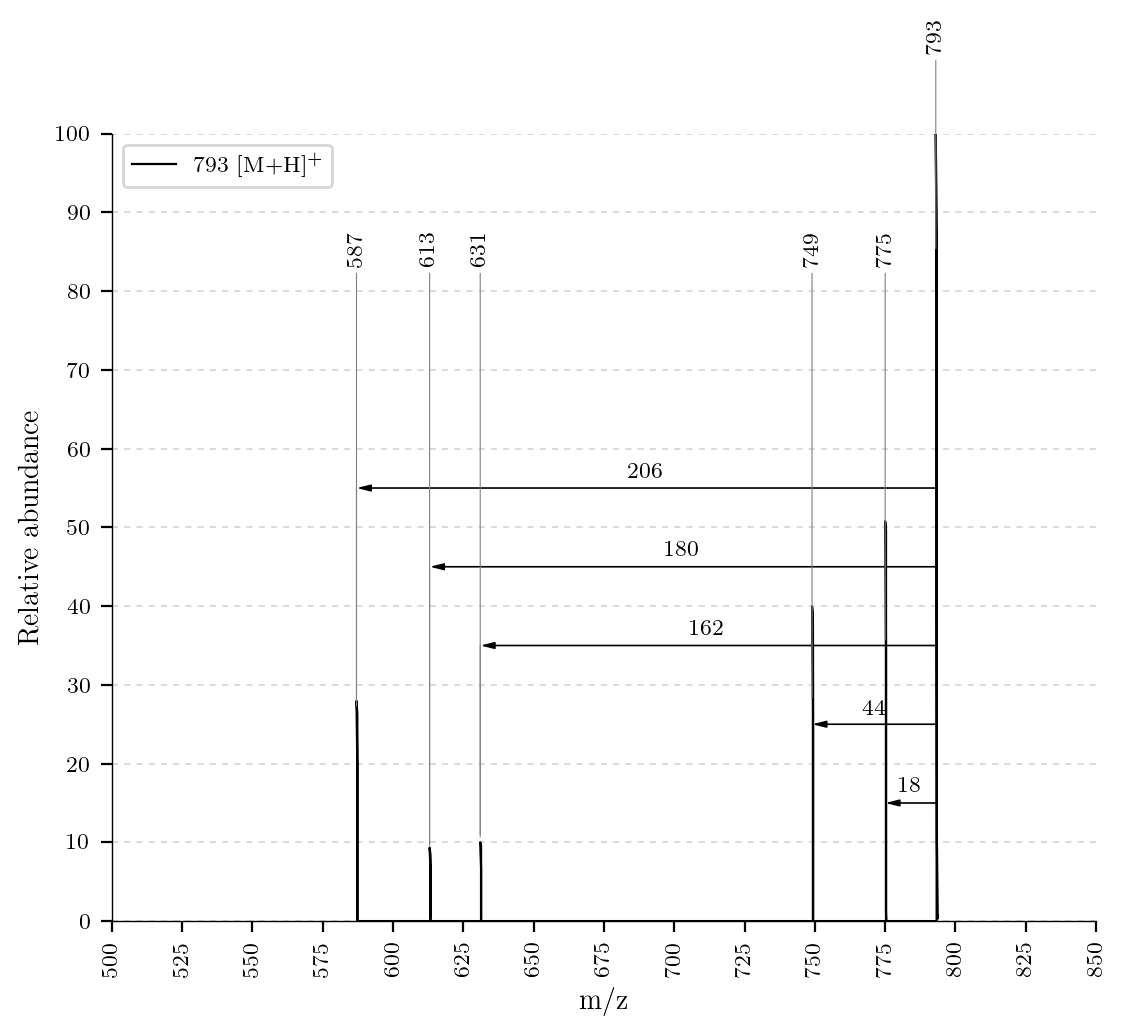
\includegraphics[width=\textwidth, height=0.7\textwidth]{figures/Kapitel7/Kataboliten/VWA_MS_793.png}
  \caption[ESI-MS Spektrum von Bo-NCC-1, Quelle: Autor]{ESI-MS Spektrum von Bo-NCC-1}
  \label{fig:793MH}
\end{figure}



\section{Reaktionsprodukte der Chl-Kataboliten}

\subsection{Reaktionsprodukt von Bo-DYCC}

Vom Bo-DYCC konnten zwei Reaktionsprodukte gefunden werden, eines bei m/z = 631 und eines bei m/z = 645. Beim ersten entsteht ein Methylester. Dieser wird an Position .. vermutet, da das Ion eine Abspaltung von \ch{CO2} bei m/z = 587 zeigt (Abbildung \ref{fig:645MH}). Beim Reaktionsprodukt bei m/z = 645 enstehen zwei Methylester, an den Positionen .. und .. .  Dies zeigt die Abspaltung von \gls{meoh} bei 613 (Abbildung \ref{fig:631MH}). 

Dies ist überraschend, da bei den meisten anderen untersuchten \gls{Chl-K} die Bildung eines Monomethylesters an Position beobachtet wurde.

\begin{figure}[!htbp]
  \centering
  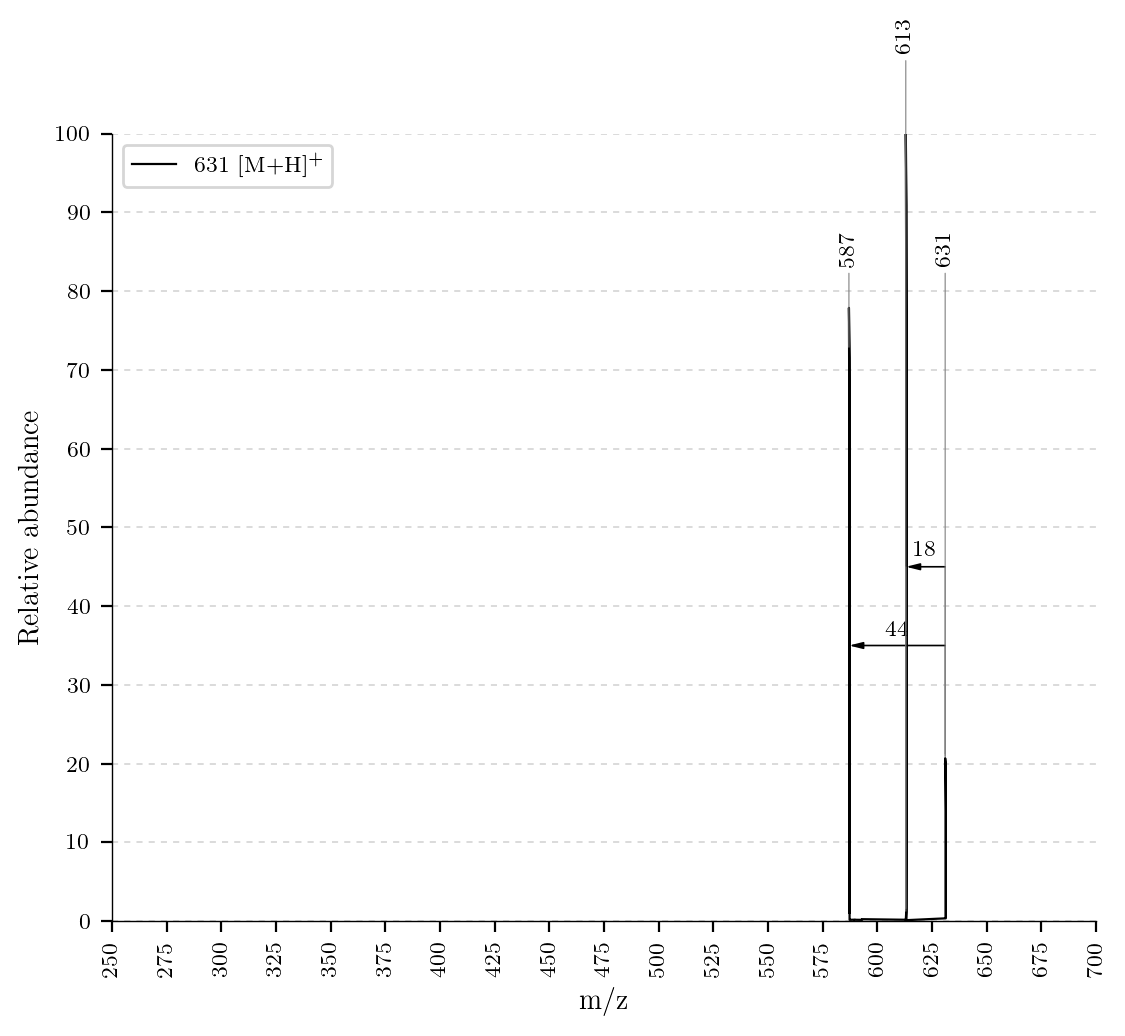
\includegraphics[width=\textwidth, height=0.7\textwidth]{figures/Kapitel7/Kataboliten/VWA_MS_631.png}
  \caption[ESI-MS Spektrum des Monomethylesters von Bo-DYCC, Quelle: Author]{ESI-MS Spektrum des Monomethylesters von Bo-DYCC bei m/z = 631}
  \label{fig:631MH}
\end{figure}

\begin{figure}[!htbp]
  \centering
  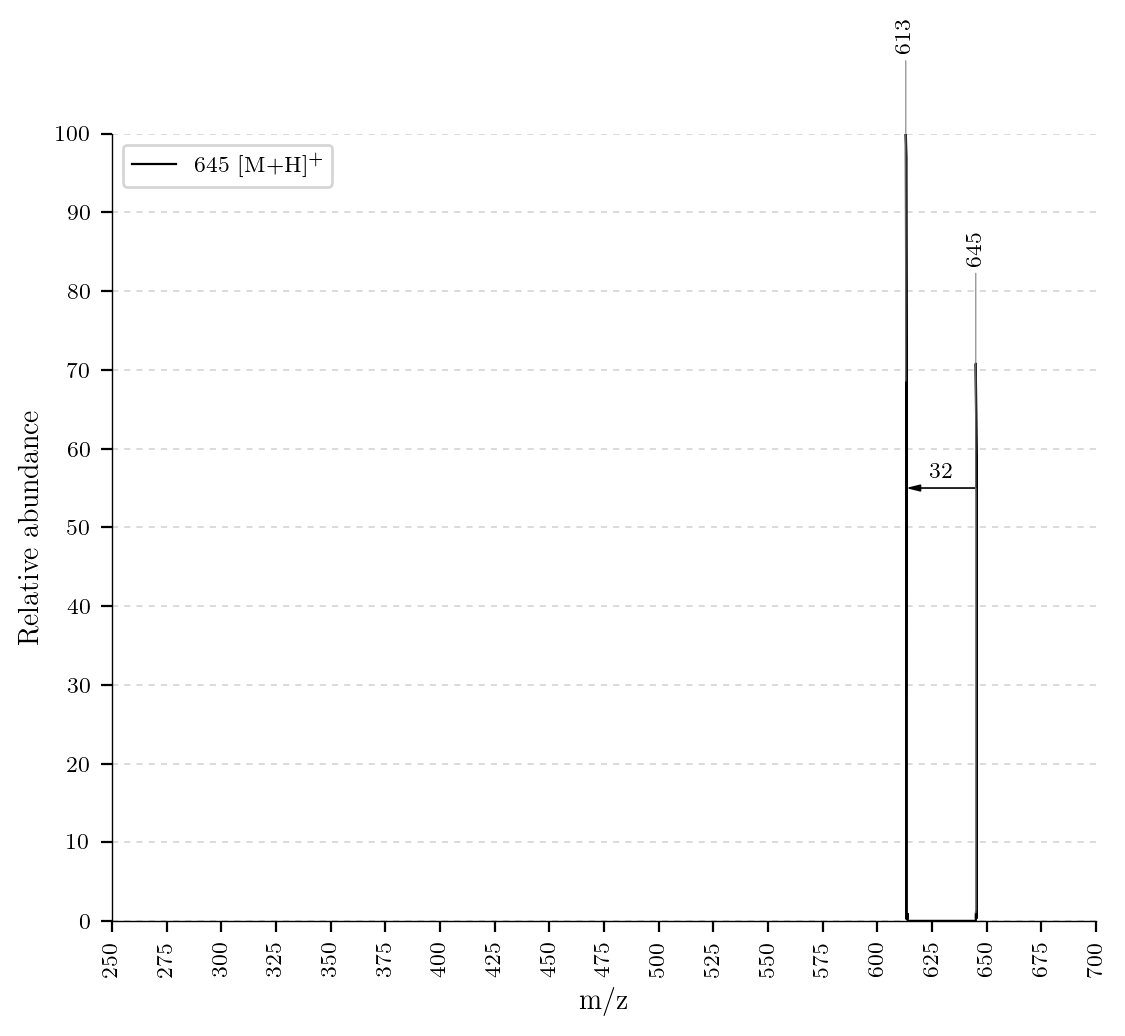
\includegraphics[width=\textwidth, height=0.6\textwidth]{figures/Kapitel7/Kataboliten/VWA_MS_645-2.png}
  \caption[ESI-MS Spektrum des Diethylesters von Bo-DYCC, Quelle: Author]{ESI-MS Spektrum des Diethylesters von Bo-DYCC bei m/z = 645}
  \label{fig:645MH}
\end{figure}


\begin{figure}[!htbp]
  \begin{subfigure}[b]{0.5\textwidth}
    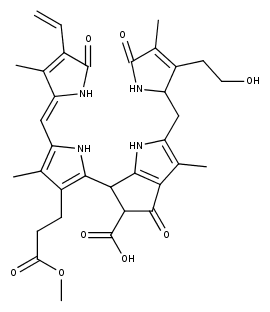
\includegraphics[width=\textwidth]{figures/Kapitel7/Kataboliten/fragmentation_structures/VWA_Katabolit_631.png}
    \caption{}
    \label{fig:631MHStruktur}
  \end{subfigure}
  \hfill
  \begin{subfigure}[b]{0.5\textwidth}
    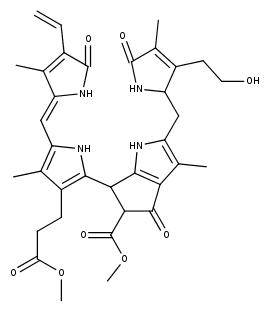
\includegraphics[width=\textwidth]{figures/Kapitel7/Kataboliten/fragmentation_structures/VWA_Katabolit_645_nachReaktion.png}
    \caption{}
    \label{fig:645MHStruktur}
  \end{subfigure}
  \caption[Strukturvorschläge für das Mono- und Dimethylierungsprodukt des Bo-DYCC, Quelle: Autor]{(a) Strukturvorschlag für das Monomethylierungsprodukt des Bo-DYCC mit Summenformel \ch{}, (b) Strukturvorschlag für das Dimethlyierungsprodukt des Bo-DYCC mit Summenformel \ch{}}
\end{figure}

\subsection{Reaktionsprodukt von Bo-DNCC}

Das Reaktionsprodukt des Bo-DNCC wurde bei m/z = 633 gefunden. Aufgrund der Abspaltung von \ch{meoh} wird angenommen, dass sich der Methylester an Position .. ausbildet.

\begin{figure}[!htbp]
  \centering
  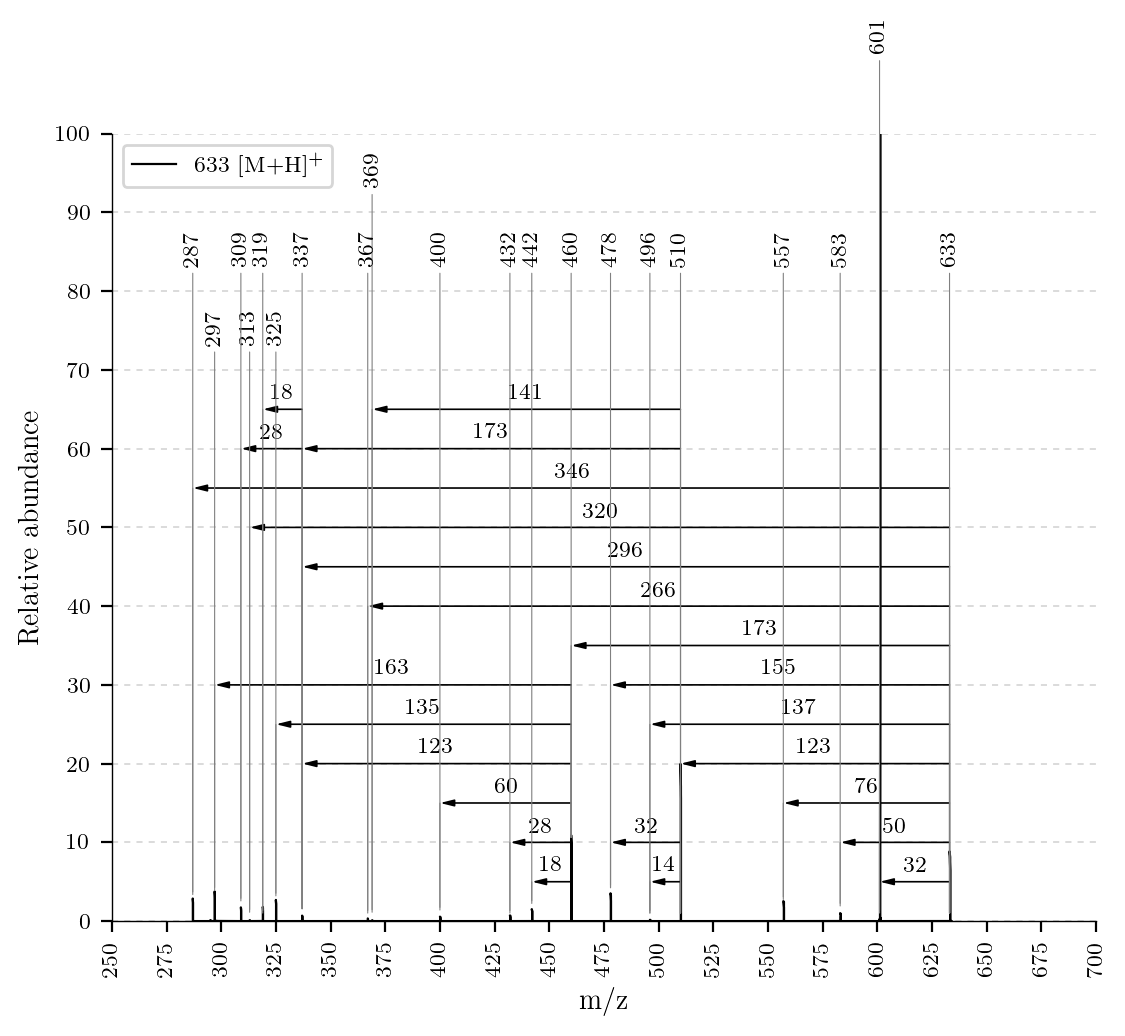
\includegraphics[width=\textwidth, height=0.7\textwidth]{figures/Kapitel7/Kataboliten/VWA_MS_633.png}
  \caption[ESI-MS Spektrum des Reaktionsproduktes von Bo-DNCC, Quelle: Autor]{ESI-MS Spektrum des Reaktionsproduktes des Bo-DNCC}
  \label{fig:633MH}
\end{figure}

\begin{figure}[!htbp]
  \centering
  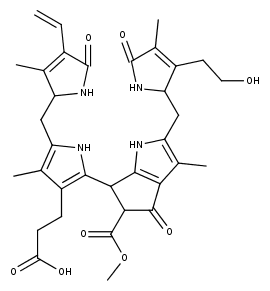
\includegraphics[scale=0.6]{figures/Kapitel7/Kataboliten/fragmentation_structures/VWA_Katabolit_633.png}
  \caption[LC-MS Chromatogramm vor der Reaktion, Quelle: Autor]{Strukturvorschlag für das Reaktionsprodukt von Bo-DNCC mit Summenformel \ch{}}
  \label{fig:633MStruktur}
\end{figure}

\subsection{Reaktionsprodukt von Bo-YCC}

Das Reaktionsprodukt des Bo-DYCC konnte nicht gesammelt werden, weswegen keine weiteren strukturellen Informationen vorhanden sind. Es wurde lediglich im \gls{lcms} Lauf identifiziert.

\subsection{Reaktionsprodukt von Bo-NCC-3}

Das Reaktionsprodukt des Bo-NCC-3 konnte bei m/z = 661 identifiziert werden und zeigt sich, so wie das Reaktionsprodukt von Bo-DNCC als sehr fragmentierungsfreudig (Abbildung \ref{fig:661MH}). 

\begin{figure}[!htbp]
  \centering
  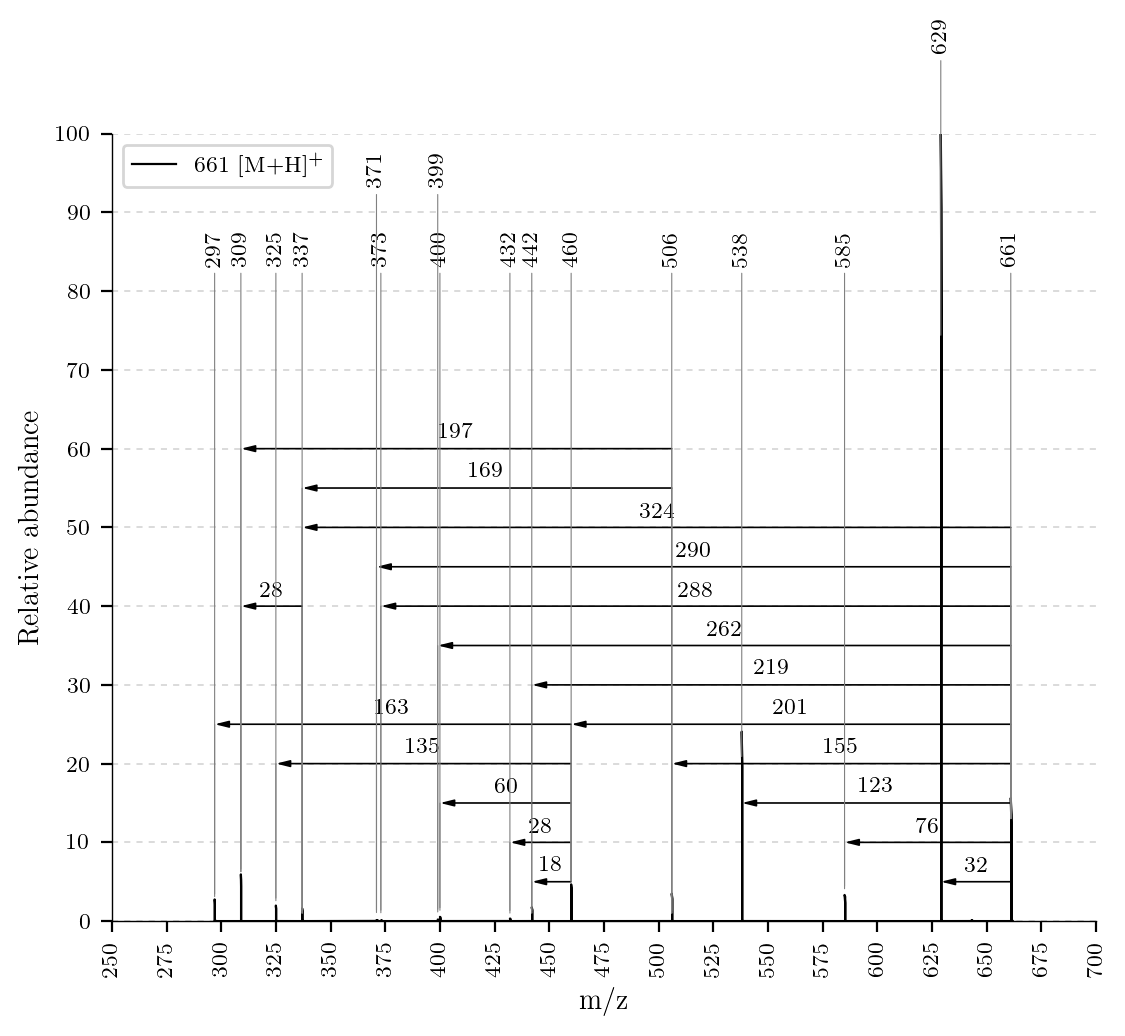
\includegraphics[width=\textwidth, height=0.7\textwidth]{figures/Kapitel7/Kataboliten/VWA_MS_661.png}
  \caption[ESI-MS des Reaktionsproduktes von Bo-NCC-3, Quelle: Author]{ESI-MS des Reaktionsproduktes von Bo-NCC-3 bei m/z = 661}
  \label{fig:661MH}
\end{figure}

\subsection{Reaktionsprodukt von Bo-NCC-1}

Das Reaktionsprodukt des Bo-NCC-1 konnte ebenfalls nicht gesammelt werden. Es wurde aber im \gls{lcms} identifiziert.
